%% LyX 2.3.6.1 created this file.  For more info, see http://www.lyx.org/.
%% Do not edit unless you really know what you are doing.
\documentclass[english]{article}
\usepackage[T1]{fontenc}
\usepackage[latin9]{luainputenc}
\usepackage{geometry}
\geometry{verbose,tmargin=2.5cm,bmargin=2.5cm,lmargin=2.5cm,rmargin=2.5cm}
\usepackage{array}
\usepackage{calc}
\usepackage{textcomp}
\usepackage{multirow}
\usepackage{graphicx}
\PassOptionsToPackage{normalem}{ulem}
\usepackage{ulem}

\makeatletter

%%%%%%%%%%%%%%%%%%%%%%%%%%%%%% LyX specific LaTeX commands.
%% Because html converters don't know tabularnewline
\providecommand{\tabularnewline}{\\}

\makeatother

\usepackage{babel}
\begin{document}
{[}SPLIT\_HERE{]}
\begin{enumerate}
\item \textbf{{[}ACJC/PRELIM/9569/2021/P2/Q1{]} }

\noindent The Universal Product Code (UPC) system is used for tracking
trade items in shipping, inventory, and sales. Each item is given
a 12-digit identification number. The validity of this identification
number can be checked using a checksum. If $x_{i}$ represents the
$i$th digit (starting with $i=1$ as the leftmost digit), then a
valid identification number satisfies the condition that

\noindent 
\[
3x_{1}+x_{2}+3x_{3}+x_{4}+3x_{5}+x_{6}+3x_{7}+x_{8}+3x_{9}+x_{10}+3x_{11}+x_{12}
\]

\noindent has a remainder of 0 when divided by 10.

\noindent The identification number can be encoded into a barcode.
For this Task, the barcode will be represented as a string of '\texttt{0}'s
and '\texttt{1}'s, where '\texttt{0}' represents a white stripe and
'\texttt{1}' represents a black stripe.

\noindent The barcode is divided into seven sections. From left to
right, they are
\begin{itemize}
\item A \textquoteleft quiet zone\textquoteright{} consisting of nine '\texttt{0}'s; 
\item A start pattern which is always '\texttt{101}'; 
\item The first six digits of the identification number are encoded using
the table below; 
\item A middle pattern which is always '\texttt{01010}'; 
\item The last six digits of the identification number are encoded using
the table below; 
\item An end pattern which is always '\texttt{101}'; 
\item A \textquoteleft quiet zone\textquoteright{} consisting of nine '\texttt{0}'s.
\end{itemize}
\noindent The table below shows the encoding system for the digits.
Note that depending on whether the digit occurs in the first six digits
or the last six digits, it would be encoded differently. However,
the two encodings are optical inverses of each other -- a '\texttt{0}'
is changed into a '\texttt{1}', and vice versa.
\noindent \begin{center}
\begin{tabular}{|c|c|c|}
\hline 
Digit  & First six digits & Last six digits\tabularnewline
\hline 
0  & \texttt{'0001101' } & \texttt{'1110010'}\tabularnewline
\hline 
1  & \texttt{'0011001' } & \texttt{'1100110'}\tabularnewline
\hline 
2  & \texttt{'0010011'} & \texttt{'1101100'}\tabularnewline
\hline 
3  & \texttt{'0111101' } & \texttt{'1000010' }\tabularnewline
\hline 
4  & \texttt{'0100011' } & \texttt{'1011100' }\tabularnewline
\hline 
5  & \texttt{'0110001' } & \texttt{'1001110'}\tabularnewline
\hline 
6  & \texttt{'0101111' } & \texttt{'1010000'}\tabularnewline
\hline 
7  & \texttt{'0111011'} & \texttt{'1000100' }\tabularnewline
\hline 
8  & \texttt{'0110111' } & \texttt{'1001000'}\tabularnewline
\hline 
9  & \texttt{'0001011' } & \texttt{'1110100'}\tabularnewline
\hline 
\end{tabular}
\par\end{center}

\noindent The reason for encoding the first and last six digits differently
is that the barcode may inadvertently be scanned upside down. Notice
that in the first six digits, the encoding for each digit contains
an odd number of '\texttt{1}'s, while in the last six digits, the
encoding for each digit contains an even number of '\texttt{1}'s.
This allows the scanning software to detect if the barcode has been
placed upside down and correct it. \quad{} 

\noindent For example, the UPC identification number 036000 291452
would be encoded as:

\begin{tabular}{|c|c|c|c|c|c|}
\hline 
000000000 & 101 & 0001101 & 0111101 & 0101111 & 0001101\tabularnewline
\hline 
Quiet & Start & 0 & 3  & 6  & 0\tabularnewline
\hline 
\end{tabular}

\begin{tabular}{|c|c|c|c|c|c|}
\hline 
0001101  & 0001101  & 01010 & 1101100  & 1110100  & 1100110\tabularnewline
\hline 
0  & 0  & Middle & 2  & 9  & 1\tabularnewline
\hline 
\end{tabular}

\begin{tabular}{|c|c|c|c|c|}
\hline 
1011100 & 1001110  & 1101100  & 101 & 000000000 \tabularnewline
\hline 
4  & 5  & 2  & End & Quiet\tabularnewline
\hline 
\end{tabular}
\noindent \begin{center}
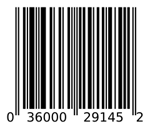
\includegraphics[scale=0.8]{C:/Users/Admin/Desktop/Github/question_bank/LyX/static/img/9597-ACJC-2021-P2-Q1}
\par\end{center}

\noindent (Notice that in an actual barcode, the stripes for the start,
middle and end pattern are usually slightly longer than the surrounding
stripes. This is to help humans to read it.)

\subsection*{Task 1.1}

\noindent Write a function to determine the validity of any input
string as an identification number. \hfill{}{[}5{]}

\subsection*{Task 1.2}

\noindent Write a function to convert a valid identification number,
given as a string, into a barcode (a string of '\texttt{0}'s and '\texttt{1}'s).
\hfill{}{[}5{]}

\subsection*{Task 1.3}

\noindent Write a function that takes in a string, check whether it
represents a valid barcode, and converts it to an identification number
if it does. Note that the barcode may be upside down. \hfill{}{[}11{]}

\noindent Download your program code and output for Task 1 as \texttt{TASK1\_<your
name>\_<centre number>\_<index number>.ipynb}

{[}SPLIT\_HERE{]}
\item \textbf{{[}ACJC/PRELIM/9569/2021/P2/Q2{]} }

\noindent A file compression algorithm reduces file sizes so that
files can be sent more quickly. One such algorithm is the Huffman
algorithm for text files, which will be implemented in this task.

\noindent Unlike ASCII, which assigns a fixed size of 8 bits for each
character, the Huffman algorithm assigns fewer bits to more common
characters and more bits to less common characters. For example, in
a long text written in English, characters such as '\texttt{e}' and
'\texttt{t}' will have fewer bits assigned to them than characters
such as '\texttt{q}' and '\texttt{z}'. If the text is long enough,
this will use fewer bits in total to encode the text compared to ASCII.

\noindent To know which sequence of bits to encode for each character,
the \textbf{frequency} of each character, which is the number of times
each character appears in the text file, is tabulated.

\noindent The characters are put into a tree. A node is created for
each character. The following steps are then repeated until there
is only one node without a parent:
\begin{enumerate}
\item Identify the two nodes, without parents, which have the lowest frequency. 
\item Create a new node whose left and right children are the two nodes
identified in Step 1. The frequency of the new node is the total of
the frequency of its children.
\end{enumerate}
\noindent The diagram on the following page shows the process of creation
of a tree for a file with only five distinct characters ('\texttt{A}',
'\texttt{E}', '\texttt{I}', '\texttt{O}' and '\texttt{U}'), in five
stages.

\noindent The bit sequence assigned to a character will be the path
from the root to the node corresponding to that character, where going
left corresponds to '\texttt{0}' and going right corresponds to '\texttt{1}'.
For example, '\texttt{A}' is encoded as '\texttt{10}' and '\texttt{O}'
is encoded as '\texttt{011}'.

\subsection*{Task 2.1}

\noindent Create a Node class that has the following attributes: 
\begin{itemize}
\item \texttt{data}, which is determined when the node is initialized 
\item \texttt{left}, a pointer to another node, 
\item \texttt{right}, a pointer to another node 
\end{itemize}
\noindent When the node is initialised, left and right do not point
to anything. The class also has setter methods for left and right,
and getter methods for all three attributes. \hfill{}{[}3{]}

\subsection*{Task 2.2}

\noindent Write code that takes an input \texttt{.txt} file and creates
a dictionary whose keys are the characters in the file, including
spaces, punctuation and line breaks ('\texttt{\textbackslash n}'),
and the value of a key is its frequency in the file. Uppercase and
lowercase letters should be considered as different characters.

\noindent Create a node for each character in the file, and put the
nodes into a list in ascending order of frequency. \hfill{}{[}11{]}

\subsection*{Task 2.3}

\noindent Create a tree using the algorithm described above. \hfill{}{[}5{]}

\subsection*{Task 2.4}

\noindent Create a dictionary whose keys are the characters, and the
value of a key is the bit sequence of that character, expressed as
a string of '\texttt{0}'s and '\texttt{1}'s.

\noindent Carry out Tasks 2.2 to 2.4 on the file \texttt{HAMLET.txt}.
Compress the file by replacing each character with its bit sequence
and writing the output to a new file, \texttt{HAMLET\_compressed.txt}.
{[}8{]}

\noindent Download your program code and output for Task 2 as \texttt{TASK2\_<your
name>\_<centre number>\_<index number>.ipynb} 

\noindent Diagram showing how the tree is created based on the frequency
of each character: 
\noindent \begin{center}
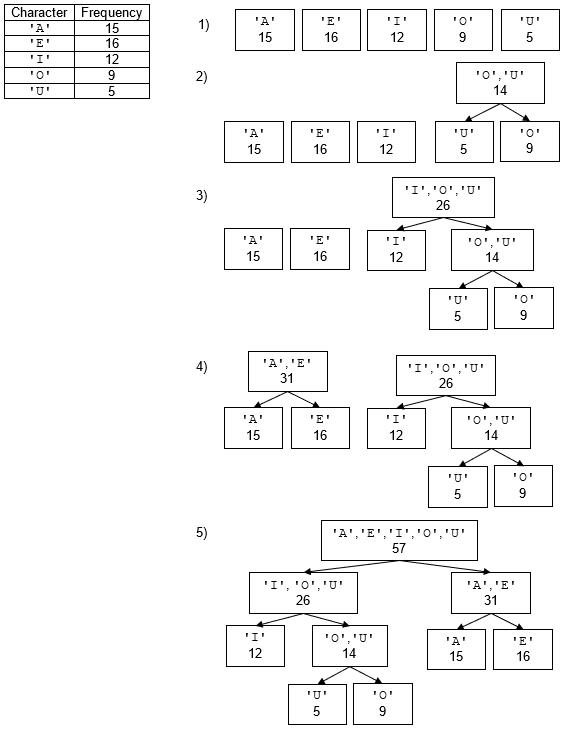
\includegraphics[scale=0.8]{C:/Users/Admin/Desktop/Github/question_bank/LyX/static/img/9597-ACJC-2021-P2-Q2}\quad{}
\par\end{center}

{[}SPLIT\_HERE{]}
\item \textbf{{[}ACJC/PRELIM/9569/2021/P2/Q3{]} }

\noindent A community centre is required to keep COVID-19 vaccination
records of its members in a NoSQL database. The CoviDie vaccine, which
requires two doses to be taken at least 21 days apart, has been secured
for all members of this particular community centre. 

\noindent As everyone needs to be vaccinated before the end of 2021,
we shall only consider the year 2021, which is a non-leap year. The
table below shows the number of days available in the twelve months
of 2021.
\noindent \begin{center}
\begin{tabular}{|c|c|c|c|c|c|c|}
\hline 
Month  & 01  & 02  & 03  & 04  & 05  & 06\tabularnewline
\hline 
Days  & 31  & 28  & 31  & 30  & 31 & 30\tabularnewline
\hline 
\end{tabular}
\par\end{center}

\noindent \begin{center}
\begin{tabular}{|c|c|c|c|c|c|c|}
\hline 
Month  & 07  & 08  & 09 & 10  & 11  & 12\tabularnewline
\hline 
Days & 31 & 31 & 30 & 31 & 30 & 31\tabularnewline
\hline 
\end{tabular}
\par\end{center}

\subsection*{Task 3.1}

\noindent Write a function \texttt{second\_dose\_date(date)} that:
\begin{itemize}
\item Takes a string value \texttt{date} in the format \texttt{YYYYMMDD},
where \texttt{YYYY} represents the year, \texttt{MM} represents the
month and \texttt{DD} represents the day 
\item determines the date that is 21 days after the input date 
\item returns the result date in the format \texttt{YYYYMMDD}
\end{itemize}
\noindent Assume that the result date does not go beyond \texttt{20211231}.
\hfill{}{[}3{]}

\noindent Test the function using the following three calls:
\begin{itemize}
\item \texttt{second\_dose\_date('20210105') }
\item \texttt{second\_dose\_date('20210212') }
\item \texttt{second\_dose\_date('20210919')} \hfill{}{[}3{]}
\end{itemize}
\noindent Save your program code as

\noindent \texttt{TASK3\_1\_<your name>\_<centre number>\_<index number>.py}

\subsection*{Task 3.2}

\noindent The list of members under the management committee of the
community centre is stored in the text file \texttt{VACCINATION.txt}.
Some members have not taken the vaccination at all, some others have
only taken the first dose, while the rest have taken both doses.

\noindent Each line of the text file is of the following format: \texttt{\_id,name,date\_first\_dose,date\_second\_dose,remarks}
\begin{itemize}
\item \texttt{\_id} is a unique integer ID assigned to the member 
\item \texttt{name} is the name of the member 
\item \texttt{date\_first\_dose} and \texttt{date\_second\_dose}, if any,
represent the date of the first dose and the date of the second dose
respectively in the format \texttt{YYYYMMDD} 
\item \texttt{remarks}, if any, shows the pre-existing condition of the
member
\end{itemize}
\noindent Write program code to insert the data from \texttt{VACCINATION.txt}
into a NoSQL database \texttt{community\_centre} under the collection
\texttt{management\_committee}. The program should clear the collection
\texttt{management\_committee} if it exists inside the database. \hfill{}{[}7{]}

\noindent Save your program code as T\texttt{ASK3\_2\_<your name>\_<centre
number>\_<index number>.py}

\subsection*{Task 3.3}

\noindent The community centre needs a program to check the vaccination
status of its members. The program should also allow for the downloading
of vaccination certificates for members who are fully vaccinated,
i.e. they have taken the two doses.

\noindent Write program code to: 
\begin{itemize}
\item prompt the user to input a member ID, and keep prompting until the
user keys in numeric character(s) 
\item if the member ID is available in the NoSQL database, perform either
one of the following: 
\begin{itemize}
\item if the member is fully vaccinated, write the vaccination certificate
to an output text file and update the record in the NoSQL database
by including a field and an appropriate value to indicate that the
certificate has been downloaded 
\item if the member has only taken the first dose, output a message to show
the date from which the member can take the second dose 
\item if the member has not taken the vaccination at all, output a message
to tell that the member should take the first dose as soon as possible 
\end{itemize}
\item otherwise, if the member ID is not available in the NoSQL database,
display an appropriate message and terminate the program
\end{itemize}
\noindent The format of the vaccination certificate is as follows.

\noindent \texttt{VACCINATION CERTIFICATE}

\noindent \texttt{Name: <name> }

\noindent \texttt{Vaccine type: CoviDie }

\noindent \texttt{Date of first dose: <date\_first\_dose> }

\noindent \texttt{Date of second dose: <date\_second\_dose>} \hfill{}{[}8{]}

\noindent Save your program code as \texttt{TASK3\_3\_<your name>\_<centre
number>\_<index number>.py}

\noindent Test your program for the member with \texttt{member\_id
= 24}. \hfill{}{[}2{]}

\noindent The output text file should be saved as \texttt{TASK3\_3\_<your
name>\_<centre number>\_<index number>.txt}

{[}SPLIT\_HERE{]}
\item \textbf{{[}ACJC/PRELIM/9569/2021/P2/Q4{]} }

\noindent A company specialising in bento boxes wishes to trial a
relational database management system to manage its data. It is expected
that the database should be normalised to third normal form (3NF).

\noindent The company owns four kiosks. For each of the kiosks, the
following information is to be recorded in the table \texttt{Kiosk}: 
\begin{itemize}
\item \texttt{KioskID} -- the unique integer assigned to the kiosk 
\item \texttt{Location} -- the area where the kiosk is located 
\item \texttt{Rating} -- the average rating of the kiosk between 0.0 and
5.0 inclusive
\end{itemize}
\noindent The company offers eight different types of bento boxes.
Some of them may contain egg, nut, seafood or a combination of them.
For each of the bento boxes, the following information is to be recorded
in the table \texttt{BentoBox}:
\begin{itemize}
\item \texttt{BentoName} -- the unique name of the bento box 
\item \texttt{ProductionCost} -- the cost incurred in producing the bento
box in dollars and cents 
\item \texttt{ContainEgg} -- an integer 0 for not containing egg and 1
for containing egg 
\item \texttt{ContainNut} -- an integer 0 for not containing nut and 1
for containing nut 
\item \texttt{ContainSeafood} -- an integer 0 for not containing seafood
and 1 for containing seafood 
\end{itemize}
\noindent Each of the four kiosks sells all eight bento boxes at different
mark-up prices. Another table \texttt{KioskBento} is needed to record
the following information:
\begin{itemize}
\item \texttt{KioskID} -- the unique integer assigned to the kiosk 
\item \texttt{BentoName} -- the unique name of the bento box 
\item \texttt{SellPrice} -- the price at which the bento box is sold at
the kiosk in dollars and cents
\end{itemize}

\subsection*{Task 4.1}

\noindent Create an SQL file called \texttt{TASK4\_1\_<your name>\_<centre
number>\_<index number>.sql} to show the SQL code to create the database
\texttt{bento\_company.db} with the three tables. \hfill{}{[}5{]}

\noindent Save your SQL code as \texttt{TASK4\_1\_<your name>\_<centre
number>\_<index number>.sql}

\subsection*{Task 4.2}

\noindent The files \texttt{KIOSK.txt} and \texttt{BENTOBOX.txt} contain
information about the company\textquoteright s kiosks and bento boxes
respectively for insertion into the database. Each row in the two
files is a comma-separated list of information. 

\noindent For \texttt{KIOSK.txt}, information about each kiosk is
given in the following order: \texttt{KioskID}, \texttt{location},
\texttt{rating}

\noindent For \texttt{BENTOBOX.txt}, information about each bento
box is given in the following order: \texttt{BentoName}, \texttt{ProductionCost},
\texttt{ContainEgg}, \texttt{ContainNut}, \texttt{ContainSeafood}

\noindent The mark-up price for each kiosk has been set as follows:
\begin{itemize}
\item \texttt{KioskID = 1} sells each bento box at a price that is \$2.60
higher than the production cost
\item \texttt{KioskID = 2} sells each bento box at a price that is \$2.90
higher than the production cost 
\item \texttt{KioskID = 3} sells each bento box at a price that is \$2.40
higher than the production cost 
\item \texttt{KioskID = 4} sells each bento box at a price that is \$3.10
higher than the production cost
\end{itemize}
\noindent Write program code to insert all the required information
into the database \texttt{bento\_company.db}. \hfill{}{[}6{]}

\noindent Save your program code as \texttt{TASK4\_2\_<your name>\_<centre
number>\_<index number>.py}

\noindent Run your program.

\subsection*{Task 4.3}

\noindent The company wishes to create a form to display the bento
boxes sold at a particular kiosk and their prices in a web browser.
The form should allow customers to indicate egg, nut and seafood allergies,
if any, and filter out the bento boxes that they cannot consume.

\noindent Write a Python program and the necessary files to create
a web application that:
\begin{itemize}
\item receives input from a HTML form that includes:
\begin{itemize}
\item a text box to enter the \texttt{location} of the kiosk 
\item three checkboxes to indicate egg, nut and seafood allergies, if any
\end{itemize}
\item returns a HTML document to display only the bento boxes that the customers
can consume based on the allergies indicated, if any, and their prices
for the given \texttt{location}
\end{itemize}
\noindent Input validation is not required. \hfill{}{[}10{]}

\noindent Save your Python program as \texttt{TASK4\_3\_<your name>\_<centre
number>\_<index number>.py}

\noindent with any additional files / sub-folders as needed in a folder
named \texttt{TASK4\_3\_<your name>\_<centre number>\_<index number>}

\noindent Run and test the web application using the following input:
\begin{itemize}
\item \texttt{'Woodlands'} entered as the \texttt{location} 
\item checkboxes indicating egg and seafood allergies ticked \hfill{}{[}2{]}
\end{itemize}
\noindent Save the output of the program as \texttt{TASK4\_3\_<your
name>\_<centre number>\_<index number>.html }

{[}SPLIT\_HERE{]}
\item \textbf{{[}ACJC/PRELIM/9569/2021/P1/Q1{]} }

A famous restaurant only accommodates one seating daily from 6.00
pm to 8.00 pm. It has 10 tables, each with a maximum capacity between
2 and 8 people. Advanced reservation is required to dine in at the
restaurant. 

The owner of the restaurant decides to write a program to handle reservations.
As a trial, it can only take a booking for one evening only. 

A procedure to initialise the arrays \texttt{MaxSize}, \texttt{IsBooked}
and \texttt{GroupSize} has been defined. The indexes of each array
corresponds to the table number.

\begin{tabular}{|c|c|}
\multicolumn{1}{c}{Index} & \multicolumn{1}{c}{\texttt{MaxSize}}\tabularnewline
\hline 
1 & 2\tabularnewline
\hline 
2 & 2\tabularnewline
\hline 
3 & 4\tabularnewline
\hline 
4 & 4\tabularnewline
\hline 
5 & 4\tabularnewline
\hline 
6 & 6\tabularnewline
\hline 
7 & 6\tabularnewline
\hline 
8 & 6\tabularnewline
\hline 
9 & 8\tabularnewline
\hline 
10 & 8\tabularnewline
\hline 
\end{tabular}%
\begin{tabular}{|c|c|}
\multicolumn{1}{c}{} & \multicolumn{1}{c}{\texttt{IsBooked}}\tabularnewline
\hline 
1 & FALSE\tabularnewline
\hline 
2 & FALSE\tabularnewline
\hline 
3 & FALSE\tabularnewline
\hline 
4 & FALSE\tabularnewline
\hline 
5 & FALSE\tabularnewline
\hline 
6 & FALSE\tabularnewline
\hline 
7 & FALSE\tabularnewline
\hline 
8 & FALSE\tabularnewline
\hline 
9 & FALSE\tabularnewline
\hline 
10 & FALSE\tabularnewline
\hline 
\end{tabular}%
\begin{tabular}{|c|c|}
\multicolumn{1}{c}{} & \multicolumn{1}{c}{\texttt{GroupSize}}\tabularnewline
\hline 
1 & \tabularnewline
\hline 
2 & \tabularnewline
\hline 
3 & \tabularnewline
\hline 
4 & \tabularnewline
\hline 
5 & \tabularnewline
\hline 
6 & \tabularnewline
\hline 
7 & \tabularnewline
\hline 
8 & \tabularnewline
\hline 
9 & \tabularnewline
\hline 
10 & \tabularnewline
\hline 
\end{tabular}

The procedure \texttt{BookTable} is shown below. When a booking enquiry
is made, the number of customers is keyed in. 

\fbox{\begin{minipage}[t]{0.8\columnwidth}%
\texttt{01 PROCEDURE BookTable }

\texttt{02 \qquad{}DECLARE NumberOfCustomers, TableNumber : INTEGERS }

\texttt{03 \qquad{}DECLARE Found : BOOLEAN}

\texttt{04 \qquad{}INPUT NumberOfCustomers }

\texttt{05 \qquad{}TableNumber \textleftarrow{} 0 }

\texttt{06 \qquad{}FOUND \textleftarrow{} False }

\texttt{07 \qquad{}REPEAT }

\texttt{08 \qquad{}\qquad{}TableNumber \textleftarrow{} TableNumber
+ 1 }

\texttt{09 \qquad{}\qquad{}IF MaxSize{[}TableNumber{]} > NumberOfCustomers
AND IsBooked{[}TableNumber{]} = FALSE }

\texttt{10 \qquad{}\qquad{}\qquad{}THEN }

\texttt{11 \qquad{}\qquad{}\qquad{}\qquad{}Found \textleftarrow{}
TRUE }

\texttt{12 \qquad{}\qquad{}ENDIF }

\texttt{13 \qquad{}UNTIL Found = TRUE AND TableNumber = 10 }

\texttt{14 \qquad{}\qquad{}IF Found = FALSE }

\texttt{15 \qquad{}\qquad{}\qquad{}THEN }

\texttt{16 \qquad{}\qquad{}\qquad{}OUTPUT \textquotedbl No tables
with enough seats available.\textquotedbl{} }

\texttt{17 \qquad{}\qquad{}\qquad{}ELSE }

\texttt{18 \qquad{}\qquad{}\qquad{}\qquad{}GroupSize{[}TableNumber{]}
\textleftarrow{} NumberOfCustomers }

\texttt{19 \qquad{}\qquad{}\qquad{}\qquad{}OUTPUT \textquotedbl Booking
is successful! Table no:\textquotedbl , TableNumber }

\texttt{20 \qquad{}ENDIF }

\texttt{21 ENDPROCEDURE}%
\end{minipage}}
\begin{enumerate}
\item There are two errors and one missing line of code in the procedure
above.
\begin{enumerate}
\item Name the type of the errors. \hfill{}{[}1{]}
\item Describe the errors and the changes required to correct them. \hfill{}{[}3{]}
\item Write the missing line of code and state where it should be located.
\hfill{}{[}2{]}
\end{enumerate}
\item Once the procedure \texttt{BookTable} is able to run correctly, the
owner decides to improve its functionality.

The procedure should ask the user to input the name and the mobile
number of the person making the reservation when a table with enough
seats can be found.

Name and describe two data validation techniques that can be applied
to any of the inputs mentioned above.\hfill{} {[}2{]}
\item Explain the difference in the type of memory allocation for an array
and a linked list. \hfill{}{[}2{]}
\end{enumerate}
{[}SPLIT\_HERE{]}
\item \textbf{{[}ACJC/PRELIM/9569/2021/P1/Q2{]} }

A hash table has 8 spaces to store strings, indexed from 1 to 8 inclusive.

The hash function finds the ASCII number of the first letter of the
string, then counts the number of 1s in its binary representation.
This is the index in which the string will be inserted into the hash
table.

For example, the string \texttt{'Arlington'} will have index 2 because
the ASCII number of '\texttt{A}' is 65, which is \texttt{1000001}
in binary, and there are two \texttt{1}s.

The following strings are to be inserted into the hash table in the
order given.

\texttt{'Grover', }

\texttt{Horsburgh', }

\texttt{'Island',}

\texttt{'Jordan', }

\texttt{'Kalman'}
\begin{enumerate}
\item Find the output of the hash function for each of the strings. \hfill{}{[}5{]}
\item {}
\begin{enumerate}
\item Suppose collisions in the hash table are to be resolved using open
hashing.

Draw the hash table after all five strings are inserted. \hfill{}{[}5{]}
\item Suppose instead that collisions in the hash table are to be resolved
using closed hashing, where spaces 6 to 8 (inclusive) are used as
the overflow storage.

Draw the hash table after all five strings are inserted. \hfill{}
{[}2{]}
\end{enumerate}
\item Explain why the space with index 1 in the hash table will never be
occupied unless there is a collision. \hfill{} {[}2{]}
\end{enumerate}
{[}SPLIT\_HERE{]}
\item \textbf{{[}ACJC/PRELIM/9569/2021/P1/Q3{]} }

The diagram below shows a flowchart for performing a search through
a binary tree. The algorithm searches through \texttt{Tree} for \texttt{Searchfor}.
If it finds a node whose data is equal to \texttt{Searchfor}, it outputs
\texttt{Found}. Otherwise, it outputs \texttt{Not Found}.
\noindent \begin{center}
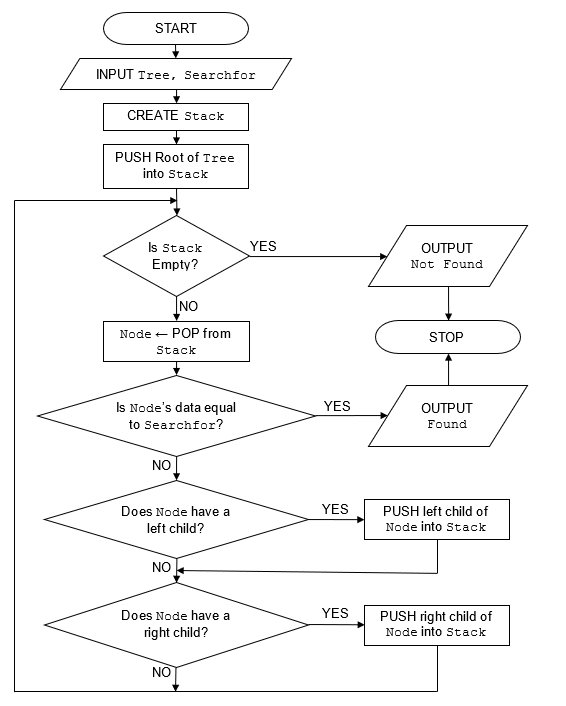
\includegraphics[scale=0.8]{C:/Users/Admin/Desktop/Github/question_bank/LyX/static/img/9597-ACJC-2021-P1-Q3-1}\quad{}
\par\end{center}
\begin{enumerate}
\item Given the input \texttt{Tree} below and a \texttt{Searchfor} value
of 5, draw a trace table to illustrate the algorithm. \hfill{} {[}5{]}
\noindent \begin{center}
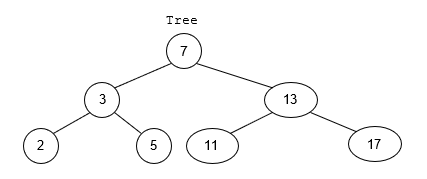
\includegraphics[scale=0.8]{C:/Users/Admin/Desktop/Github/question_bank/LyX/static/img/9597-ACJC-2021-P1-Q3-2}\quad{}
\par\end{center}
\item State whether this is a depth-first search or a breadth-first search.
\hfill{} {[}1{]}
\item Draw a flowchart to illustrate how the other kind of search in (ii)
can be carried out using the same input parameters. \hfill{} {[}3{]}
\item Given the same input \texttt{Tree} and the same \texttt{Searchfo}r
value of 5, draw a trace table to illustrate the algorithm in (iii).
\hfill{} {[}5{]}
\end{enumerate}
{[}SPLIT\_HERE{]}
\item \textbf{{[}ACJC/PRELIM/9569/2021/P1/Q4{]} }

Merge sort and bubble sort are two sorting algorithms that can be
applied to sort a list of integers in ascending order.
\begin{enumerate}
\item By briefly comparing the operation of merge sort and bubble sort,
state which algorithm would be more efficient. \hfill{}{[}3{]}
\end{enumerate}
The pseudocode for the recursive \texttt{MergeSortDesc} function is
shown below, which takes in a list of integers and returns a new list
with the integers sorted in descending order. It makes use of the
\texttt{MergeDesc} function in line \texttt{10} that merges two lists
of integers sorted in descending order into a single list of integers
sorted in descending order as well.

\fbox{\begin{minipage}[t]{0.8\columnwidth}%
\texttt{01 FUNCTION MergeSortDesc(MyList: LIST) RETURNS LIST }

\texttt{02 \qquad{}MaxIndex \textleftarrow{} LENGTH(MyList) }

\texttt{03 \qquad{}\qquad{}IF ......A...... }

\texttt{04 \qquad{}\qquad{}\qquad{}THEN }

\texttt{05 \qquad{}\qquad{}\qquad{}Half \textleftarrow{} ......B...... }

\texttt{06 \qquad{}\qquad{}\qquad{}LeftList \textleftarrow{} LEFT(MyList,
Half) }

\texttt{07 \qquad{}\qquad{}\qquad{}RightList \textleftarrow{} RIGHT(MyList,
Half) }

\texttt{08 \qquad{}\qquad{}\qquad{}SortedLeftList \textleftarrow{}
MergeSortDesc(LeftList) }

\texttt{09 \qquad{}\qquad{}\qquad{}SortedRightList \textleftarrow{}
MergeSortDesc(RightList) }

\texttt{10 \qquad{}\qquad{}\qquad{}Result \textleftarrow{} MergeDesc(SortedLeftList,
SortedRightList) }

\texttt{11 \qquad{}\qquad{}ELSE }

\texttt{12 \qquad{}\qquad{}\qquad{}......C...... }

\texttt{13 \qquad{}\qquad{}ENDIF }

\texttt{14 \qquad{}\qquad{}RETURN Result }

\texttt{15 ENDFUNCTION}%
\end{minipage}}
\begin{enumerate}
\item[(b)] State what is meant by a \textbf{recursive} function. \hfill{}{[}2{]}
\item[(c)] Write the pseudocode for \texttt{A}, \texttt{B} and \texttt{C} in
the algorithm. \hfill{}{[}3{]}
\item[(d)] Describe the operation of the \texttt{MergeDesc} function.

Assume that the function does not modify the two input lists.\hfill{}
{[}4{]}
\end{enumerate}
{[}SPLIT\_HERE{]}
\item \textbf{{[}ACJC/PRELIM/9569/2021/P1/Q5{]} }

A gym organises various classes and runs a loyalty membership programme
with four tiers: Bronze, Silver, Gold and Diamond 

Upon joining, each member is given a unique membership number and
starts with a Bronze membership. Each member can sign up for multiple
classes at a reduced rate based on the membership tier.

Each class has a unique class name. Some classes are offered at three
different levels: Beginner, Intermediate and Advanced

Each instructor is identified with a unique three-character code and
can take one or more classes.

A relational database is to be created to store data about members,
employees and classes.

Part of the table \texttt{MEMBER}, which is a first attempt at the
database design, is shown below. 

\begin{tabular}{|c|c|c|c|c|}
\hline 
MemberNo  & MemberName  & MemberTier  & ClassName & InstCode\tabularnewline
\hline 
\multirow{3}{*}{5 } & \multirow{3}{*}{Lindy White} & \multirow{3}{*}{Silver } & Body Pump  & WAY \tabularnewline
\cline{4-5} \cline{5-5} 
 &  &  & Yoga (Beginner)  & DAV \tabularnewline
\cline{4-5} \cline{5-5} 
 &  &  & Zumba & ROG\tabularnewline
\hline 
\dots{}  & \dots{}  & \dots{}  & \dots{}  & ...\tabularnewline
\hline 
78  & Derek Davis  & Bronze  & Muay Thai (Beginner)  & CHA \tabularnewline
\hline 
\dots{} & \dots{}  & \dots{} \dots{} \dots{}  & \dots{}  & ...\tabularnewline
\hline 
\multirow{4}{*}{132} & \multirow{4}{*}{John Chua } & \multirow{4}{*}{Diamond } & Circuits (Intermediate)  & JON \tabularnewline
\cline{4-5} \cline{5-5} 
 &  &  & Muay Thai (Intermediate)  & LEX \tabularnewline
\cline{4-5} \cline{5-5} 
 &  &  & Yoga (Advanced) & DAV \tabularnewline
\cline{4-5} \cline{5-5} 
 &  &  & Zumba & ROG\tabularnewline
\hline 
\dots{}  & \dots{} & \dots{}  & \dots{}  & \dots{}\tabularnewline
\hline 
\end{tabular}
\begin{enumerate}
\item The table \texttt{MEMBER} is not normalised.
\begin{enumerate}
\item Describe \textbf{one} potential issue that may be encountered when
the data are maintained in such a non-normalised table. \hfill{}{[}1{]}
\item Explain why the table is not in first normal form (1NF). \hfill{}{[}1{]}
\end{enumerate}
\item A second attempt at the database design gives rise to two tables:

\texttt{MEMBER(MemberNo, MemberName, MemberTier)}

\texttt{MEMBERCLASSES(MemberNo, ClassName, Instructor)}

The primary keys are not shown. 
\begin{enumerate}
\item State what is meant by a \textbf{primary key}. \hfill{}{[}1{]}
\item By referring to the relationship between the tables \texttt{MEMBER}
and \texttt{MEMBERCLASSES}, state how the relationship is implemented.\hfill{}
{[}2{]}
\item Write an SQL query to create the table MEMBER with the appropriate
constraints.\hfill{} {[}4{]}
\end{enumerate}
\item Another attempt at the database design needs to be made to ensure
that all the tables are in third normal form (3NF). 

In addition, the following data need to be recorded in the database:
\begin{itemize}
\item the date on which each member signs up for the gym membership; 
\item the attendance of each member in any classes taken;
\item the original fee, i.e. before discount, of each class; 
\item the name and the salary of each instructor. 
\end{itemize}
\begin{enumerate}
\item State the total number of 3NF tables required and give their names.
\hfill{}{[}1{]}
\item Draw the Entity-Relationship (E-R) diagram to show the 3NF tables
and the relationships between them. \hfill{}{[}4{]}
\item A table description can be written as:

\texttt{TableName(}\texttt{\uline{Attribute1}}\texttt{, Attribute2{*},
Attribute3, ...) }

The primary key is indicated by underlining one or more attributes.
Foreign keys are indicated by using a dashed underline/asterisk. 

Using the information provided, write table descriptions for all the
3NF tables you identified in \textbf{(c)(i)}.\hfill{} {[}8{]}
\end{enumerate}
\item Making backups and archives are performed to prevent the loss of data.

Explain the difference between a backup and an archive.\hfill{} {[}2{]}
\end{enumerate}
{[}SPLIT\_HERE{]}
\item \textbf{{[}ACJC/PRELIM/9569/2021/P1/Q6{]} }

A driving simulator is programmed using Object-Oriented Programming
(OOP).

The diagram below shows a UML Class Diagram with \textbf{some} of
the classes, attributes, and methods used in the simulator.
\noindent \begin{center}
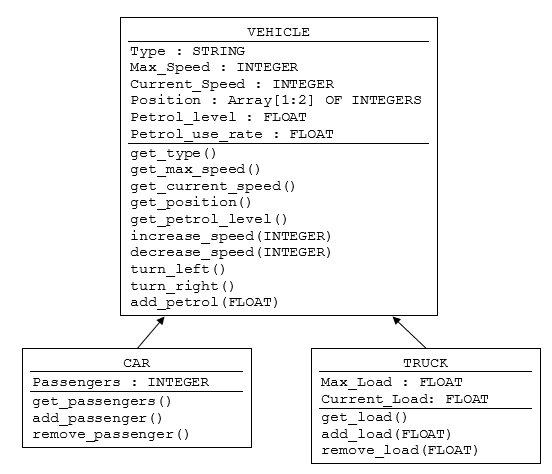
\includegraphics[scale=0.8]{C:/Users/Admin/Desktop/Github/question_bank/LyX/static/img/9597-ACJC-2021-P1-Q5}\quad{}
\par\end{center}
\begin{enumerate}
\item State the relationship between the \texttt{CAR} class and the \texttt{VEHICLE}
class. \hfill{}{[}1{]}
\item Explain briefly, in this context, how each of the following features
of Object-Oriented Programming help the simulation to be developed
more efficiently.
\begin{enumerate}
\item Abstraction \hfill{} {[}2{]}
\item Inheritance \hfill{}{[}2{]}
\end{enumerate}
\item The petrol use rate depends on the speed at which the vehicle is travelling,
as well as the mass of the vehicle and the contents of the vehicle
-- the number of passengers in a car, or the mass of the load in
a truck. Explain how polymorphism can be used in this case to write
the simulation. \hfill{}{[}2{]}
\end{enumerate}
{[}SPLIT\_HERE{]}
\item \textbf{{[}ACJC/PRELIM/9569/2021/P1/Q7{]} }

A new social media platform is to be created. In years to come, it
is expected to be as popular globally as other trending social media
platforms.
\begin{enumerate}
\item Give two reasons why a NoSQL database is likely to be more suitable
than an SQL database for the social media platform. \hfill{}{[}2{]}
\end{enumerate}
A basic login page that controls access to user accounts is shown
below. The password field masks the user input with a dot (\textbullet )
replacing each of the characters supplied.
\noindent \begin{center}
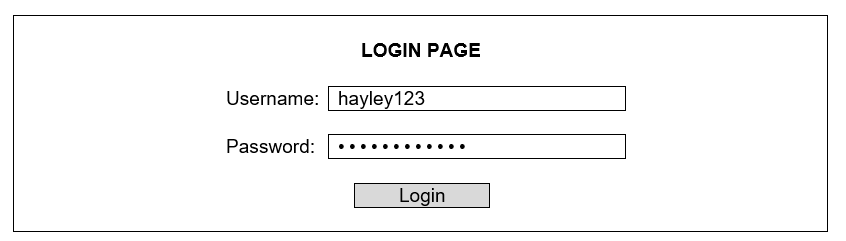
\includegraphics[scale=0.5]{C:/Users/Admin/Desktop/Github/question_bank/LyX/static/img/9597-ACJC-2021-P1-Q6}\quad{}
\par\end{center}
\begin{enumerate}
\item[(b)] When the login button is clicked, the program processes the username
and password supplied by the user.

It displays an error message if the username entered does not exist
in the database. If the password entered matches the registered password
for the username, login is granted. Otherwise, the program displays
an error message to indicate the user of the incorrect password entered.

The account will be locked if the user enters the correct username,
but enters the wrong password three times.
\begin{enumerate}
\item Create a decision table to show these conditions and actions. \hfill{}{[}4{]} 
\item Simplify your decision table by removing redundancies. \hfill{}{[}1{]} 
\end{enumerate}
\item[(c)] It is known that users tend to have different problems associated
with passwords.

Besides the error message to tell the user when an incorrect password
is entered, describe \textbf{two} examples based on usability principles
that can be applied to improve the functionality of the login page.
{[}2{]}
\item[(d)] Explain why the HTTP POST method should be used instead of the HTTP
GET method for the login request. \hfill{}{[}2{]}
\end{enumerate}
{[}SPLIT\_HERE{]}
\item \textbf{{[}ACJC/PRELIM/9569/2021/P1/Q8{]} }

In a hypothetical scenario, a data security company is helping a client
company manage a database of the client company\textquoteright s customers.
The data security company notices a possible vulnerability in the
database.

Further investigation shows that the vulnerability is obscure and
that none or few of the programmers anticipated it. Since the vulnerability
is obscure, they determine that the chances of the database being
breached are minimal, and decide not to tell the client company about
it. 

Instead, the data security company waits until the next time the database
is due for scheduled maintenance to attempt to fix the vulnerability.
By doing so, they can give themselves enough time to learn how to
fix the vulnerability and avoid causing unnecessary panic within the
client company or among the customers, which could lead to a potential
loss of business.

Describe how each of the following ethical guidelines was breached
by the data security company.
\begin{enumerate}
\item Integrity \hfill{}{[}2{]}
\item Responsibility \hfill{}{[}2{]}
\item Competence \hfill{}{[}2{]}
\item Professionalism \hfill{}{[}2{]}
\end{enumerate}
{[}SPLIT\_HERE{]}
\end{enumerate}
 
\end{document}
